\documentclass[UTF8,zihao=-4,openany,oneside]{ctexbook}
\usepackage[a4paper,left=3cm,right=2.6cm,top=3.5cm,bottom=2.6cm,headsep=0.7cm]{geometry}
\usepackage{fontspec}
\usepackage{graphicx}
\usepackage{caption}
\usepackage{booktabs}
\usepackage{array}
\usepackage{tabularx}
\usepackage{longtable}
\usepackage{setspace}
\usepackage{fancyhdr}
\usepackage{titlesec}
\usepackage{tocloft}
\usepackage{indentfirst}
\usepackage{hyperref}
\hypersetup{hidelinks}
\setmainfont{Times New Roman}
\setCJKmainfont{SimSun}
\setCJKsansfont{SimHei}
\setCJKfamilyfont{hei}{SimHei}
\providecommand{\heiti}{}
\renewcommand{\heiti}{\CJKfamily{hei}}
\setlength{\parindent}{2em}
\setlength{\parskip}{0pt}
\linespread{1.67}
\pagestyle{fancy}
\fancyhf{}
\fancyhead[C]{\zihao{5} 南京工程学院自动化学院本科毕业设计（论文）}
\fancyfoot[C]{\thepage}
\renewcommand{\headrulewidth}{0.4pt}
\ctexset{
  chapter={format=\centering\zihao{3}\heiti,beforeskip=0pt,afterskip=20pt,name={第,章},number=\chinese{chapter}},
  section={format=\zihao{4}\heiti,beforeskip=12pt,afterskip=6pt},
  subsection={format=\zihao{-4}\heiti,beforeskip=6pt,afterskip=6pt}
}
\captionsetup{font=small,labelsep=space}
\renewcommand{\contentsname}{目\quad 录}
\renewcommand{\cfttoctitlefont}{\hfill\zihao{3}\heiti}
\renewcommand{\cftaftertoctitle}{\hfill}
\renewcommand{\cftchapfont}{\zihao{-4}}
\renewcommand{\cftsecfont}{\zihao{-4}}
\renewcommand{\cftchappagefont}{\zihao{-4}}
\renewcommand{\cftsecpagefont}{\zihao{-4}}
\begin{document}
\begin{titlepage}
\thispagestyle{empty}
\centering
\vspace*{1.2cm}
{\zihao{-2}\heiti 本科生毕业论文（设计）\par}
\vspace{2.2cm}
\renewcommand{\arraystretch}{1.8}
\begin{tabular}{rl}
\zihao{4}\heiti 题目： & \underline{\makebox[9.5cm][c]{\zihao{4} 双电机同轴驱动控制系统设计}}\\
\end{tabular}
\vspace{2.0cm}
\begin{tabular}{rl}
\zihao{4}\heiti 姓   名： & \underline{\makebox[9.5cm][c]{\zihao{4} 学生姓名}}\\
\zihao{4}\heiti 学   号： & \underline{\makebox[9.5cm][c]{\zihao{4} 203220104}}\\
\zihao{4}\heiti 班   级： & \underline{\makebox[9.5cm][c]{\zihao{4} 自动化221}}\\
\zihao{4}\heiti 学   院： & \underline{\makebox[9.5cm][c]{\zihao{4} 自动化学院}}\\
\zihao{4}\heiti 专   业： & \underline{\makebox[9.5cm][c]{\zihao{4} 自动化}}\\
\zihao{4}\heiti 指导教师： & \underline{\makebox[9.5cm][c]{\zihao{4} 姓名1 姓名2}}\\
\end{tabular}
\vfill
{\zihao{4} 2026年5月\par}
\end{titlepage}
\clearpage
\begin{titlepage}
\thispagestyle{empty}
\centering
\vspace*{1.0cm}
{\zihao{3}\bfseries Graduation Design (Thesis)\par}
\vspace{1.4cm}
{\zihao{3}\bfseries Design of Dual Motor Coaxial Drive Control System\par}
\vspace{1.2cm}
{\zihao{4} By\par}
\vspace{0.35cm}
{\zihao{4} LIU Yang\par}
\vspace{0.35cm}
{\zihao{4} Supervised by\par}
\vspace{0.35cm}
{\zihao{4} CHEN Changjiang\par}
\vspace{0.35cm}
{\zihao{4} School of Automation\par}
\vspace{0.35cm}
{\zihao{4} Nanjing Institute of Technology\par}
\vspace{0.35cm}
{\zihao{4} May, 2026\par}
\vspace{0.35cm}
\end{titlepage}
\clearpage
\frontmatter
\pagenumbering{Roman}
\setcounter{page}{1}

Design of Dual Motor Coaxial Drive Control System

By

LIU Yang

Supervised by

CHEN Changjiang

School of Automation

Nanjing Institute of Technology

May, 2026

\chapter*{摘\quad 要}
\addcontentsline{toc}{chapter}{摘\quad 要}

多电机同轴驱动既能增大伺服系统的输出功率，又可消除传动链齿隙，提高系统的控制精度。现场总线具有实时性高、稳定性好等优点，广泛应用于伺服系统中，本文实现了一种基于CANopen协议的双电机同轴驱动控制系统，用于满足不同工业场合对伺服系统的输出功率和控制精度要求。

首先，本论文以STM32F407微控制器为核心，采用现场总线CANopen DS301和DSP402为通信协议，完成双电机同轴控制系统的结构框架设计、控制系统设计、控制器电路设计及制作；其次，运用Simulink建立了双电机同轴驱动仿真模型，进行双电机同轴驱动的速度、电流双闭环控制仿真，验证了双电机速度、电流双闭环PI控制算法、消隙算法的正确性，在此基础上完成了双电机同轴控制代码的编写、显示界面设计；最后，在所设计的双电机同轴控制系统硬件平台上进行实际的双电机同轴驱动的试验调试，验证了双电机同轴驱动控制算法、消隙算法等的正确性。

实验结果表明：系统架构正确，实现双电机同轴驱动控制功能，达到提高输出功率及消除传动链齿隙的目的。

\noindent\textbf{关键词：双电机；同轴驱动；CANopen协议；STM32；消隙算法}

\chapter*{ABSTRACT}
\addcontentsline{toc}{chapter}{ABSTRACT}

The dual motor coaxial drive can not only increase the output power of the servo system, but also eliminate the backlash of the drive chain to improve the control precision of the system. Field bus has the advantages of high real-time performance and good stability. It is widely used in servo system. This paper has completed a dual motor coaxial drive control system based on CANopen protocol to meet the needs of the output power and the control precision in different occasions. The structure of servo system is varied,. The main work accomplished and conclusions got are presented as follows:

First, used STM32F407 microcontroller as the control core, based on the field bus CANopen DS301 and DSP402 protocol as the communication protocol, design the framework of control system, the hardware is designed and the PCB of the system is produced. Then, based on MATLAB and Simulink the module of the dual motor coaxial drive control system is established, the speed and current double closed loop control system is simulated, the correctness of dual motor speed and current double closed loop PI control algorithm and backlash eliminating algorithm is verified. Based on that, the dual motor coaxial control software code and the display interface software are programmed. At last, the experiment is implemented on the real dual motor coaxial drive control platform, and the correctness of backlash eliminating algorithm is verified.

The experimental results show that the architecture of the system is correct, the dual motor drive control function is realized, and the purpose of increasing the output power and eliminating the backlash of the drive chain is achieved.

\noindent\textbf{Key words：Dual Motor; Coaxial Drive; CANopen Protocol; STM32; Backlash Eliminating Algorithm}

\clearpage
\tableofcontents
\clearpage
\mainmatter
\pagenumbering{arabic}
\setcounter{page}{1}
\chapter{第一章 绪 论}

\section{1.1 课题研究背景及意义}

现代工业自动化水平不断提高的同时，对工业控制伺服系统提出了更高的要求，现代伺服系统被要求能够输出较大的转矩，具备更高的定位精确度等，同时伺服驱动器被要求实现数字化，智能化和网络化。

应用中采用多电机传动的方式，可以满足不同场合的性能指标要求。全数字控制的应用使得伺服系统的控制精度和可靠性得到提高，也使系统抗干扰能力得到增强[1]（文献序号用上标，所有参考文献均须在文中标出，且按照顺序引用）。由于现场总线具有多支点、可靠性强、易扩展等特点，因此现场总线技术在伺服系统中得到了广泛应用，详细描述请参阅文献[2]（此处文献序号不用上标）。

从现代工业控制领域到军事领域甚至是航天领域，伺服系统都有着十分广泛的应用。在传统的伺服系统中，单电机的控制方式往往占据着主要角色，但是单个电机驱动系统存在不足，如在某些特殊应用场合需要较大的驱动功率时，如采用单电机驱动，不仅需求大功率的驱动电机和伺服驱动器，而且传动链的功率和体积也大大增加，不仅造成系统的成本上升，受使用环境和体积及制造工艺的限制，单电机驱动往往难以满足要求。

科学技术的不断发展，对伺服系统提出了更高的性能指标要求。对于跟踪系统来说，伺服系统的动态性能比较重要，同时需要具备较强的抗干扰能力和可靠性，能够输出高加速度；对于位置控制来说，要求伺服系统的定位精确度高；对需要大功率的场合，要求伺服系统能够平稳的驱动惯量大的负载[3]。这些场合如果采用单电机，往往不能够有效满足系统的各种性能指标的要求。伺服系统中，为了获得大转矩、低转速的效果，常采用齿轮传动，而多电机的控制方式可以消除齿轮传动中的齿隙，提高控制精度。

考虑到以上几点，多采用多电机共同驱动的方式，满足不同场合的性能指标要求。双电机驱动是一种稳定可靠的驱动方式，提高了抗干扰能力，提升了系统的响应速度，增大了驱动总功率。这种驱动系统既可以避免单电机驱动的短板，又可以消除间隙，使伺服系统响应的快速性、平稳性和精确度大幅提升[4]。这种方式不仅能够满足系统的大功率要求，而且也具备了输出大转矩的能力。

与多电机共同驱动的方式类似，双电机同轴驱动控制系统也具有诸多优势，应用的场合也越来越多，这种驱动控制系统具有的优势如下[5]：

\noindent （1）系统驱动总功率提高；\\

\noindent （2）单个电机成本降低；\\

\noindent （3）系统的通用性和可靠性提高；\\

\noindent （4）消除传动链齿隙非线性对系统的影响，控制精度提高；\\

\noindent （5）单个电机占用体积小，空间利用率高。\\

本课题采用两个参数相同的电机，共同完成驱动同一目标轴的任务，最终实现同轴驱动控制。另外考虑到复杂的工业现场环境，以及数据的实时传输和稳定通信，利用CAN总线构成了整个控制网络，并在此基础上应用了CANopen高级协议，包括DS301基础协议和针对伺服驱动设备的DSP402协议，使整个控制系统接线更加简单，数据传输更加稳定，本文完成了一种基于CANopen协议的双电机同轴驱动控制系统设计。

\section{1.2 多电机驱动控制的发展及现状}

在多电机控制系统中，需要特别注意整个系统的实时性，而现场总线在多电机控制系统中的广泛采用，使同步控制的实时性得到很大提高，数据和指令的发送也更加及时和准确，在同步控制中，CAN总线、PROFIBUS总线和CC-LINK总线等应用较广泛。同步控制的算法的发展也有了长足的进步，从1980年提出的交叉耦合器理论到各种智能控制算法，诸如遗传算法、神经网络、模糊控制等，都被运用到同步控制中，取得了不错的控制效果[6]。

在消除传动链齿隙的控制方法上，多电机控制由原来的固定输出偏置力矩变为对输出力矩实施动态控制，使得消隙控制更加完善，整个传动系统在工作过程中保持了良好的动、静态特性，提高了传动精度。

\section{1.3 现场总线技术的应用及发展}

近年来，工业数据总线的不断发展，使现场总线得到广泛应用，现场总线主要是为了解决了复杂工业环境下，工业现场设备的数据通讯和实时交换问题，也为下层现场控制设备和上层主站控制系统的信息交互提供了解决方案[7]。比如采用CAN总线实现多个伺服驱动器之间，伺服驱动器和伺服控制主站之间的信息传递。

现场总线因为具有接线简单方便、性能可靠等一系列优点，在工业控制领域以及计算机控制中受到了重视，并发挥着越来越重要的作用。现场总线的继续发展，必将为工控自动化领域带来新的活力。

\section{1.4 课题研究内容}

在了解和分析了国内外多电机驱动控制技术和实际应用中的技术指标要求后，本课题完成了一种基于CANopen协议的双电机同轴驱动控制系统，采用的CAN总线通讯技术，简化系统硬件设计。通过控制Solo Whistle数字伺服驱动器完成双电机的同轴驱动，制作人机交互界面，实现PC机和控制系统的数据传输和显示。利用数字PID技术，采用双电机电流、速度双闭环控制算法，实现系统的平稳运行，完成同轴驱动任务。本课题研究的主要内容包括：

\noindent （1）基于STM32F407微控制器的控制系统设计\\

确定双电机同轴驱动系统控制方案，依据控制系统的体系结构和功能需求确定硬件器件选型和具体实现方法，并完成相应硬件的电路设计，简要地对系统硬件各个模块的工作原理进行了阐述。

\noindent （2）CAN总线及伺服驱动的DSP402协议控制技术研究\\

在了解各种总线的特点并配合Solo Whistle数字伺服驱动器，本课题采用了CAN总线及针对伺服驱动的DSP402协议作为控制通信网络，并在STM32F407内实现CAN的底层驱动和DS301、DSP402协议，完成微控制器和两个电机驱动器之间实时数据通讯。

\noindent （3）双电机运动控制中的控制算法研究及仿真\\

在研究现有双电机同轴驱动控制算法基础上，采用单速度环控制算法实现双电机同轴驱动的力矩均衡控制，并通过偏置转矩控制实现消除传动链齿隙，提高控制系统精度。运用Simulink建立了双电机双闭环仿真模型，仿真验证了双电机双闭环算法的正确性。

\noindent （4）双电机控制系统的调试及性能测试\\

完成了双电机同轴驱动的系统硬件设计调试，并将同轴驱动控制、消隙控制算法应用到系统调试中，达到提高输出功率及消除传动链齿隙的目的。

本章主要介绍了课题的研究背景及意义，探讨了多电机驱动控制的发展及现状，分析了现场总线技术的应用及发展，最后简单介绍了课题研究的主要内容和具体包括的几个主要方面。

\chapter{第二章 控制系统总体方案设计}

注意：工程设计类的毕业设计，需要在论文中给出方案论证或方案设计。能够根据毕业设计任务对系统期望指标的要求，进行系统方案调研，确定系统总体解决方案，体现解决复杂工程问题的能力。

\section{2.1 系统总体方案确定及分析}

\subsection{2.1.1 系统总体电气结构设计}

依据课题任务要求，利用双电机实现同轴驱动控制系统设计，在查阅同轴驱动控制和现场总线等相关文献和资料基础上，确定系统控制方案，主要包括供电模块、核心板、电机驱动器、电机及显示等模块组成，系统总体结构如图2.1所示。（文章中出现的图都必须在文中引用，并且按照下列方式进行标注说明。）

\begin{center}\zihao{5}图2.1 系统总体结构框图\end{center}

\subsection{2.1.2 伺服驱动器的选择}

现代工业生产过程中对伺服系统提出了高速、高精度和高可靠性的要求。电机伺服驱动器作为伺服系统主要控制环节和输出环节，其实时性、可靠性和动态性能等方面性能的好坏往往影响到整个控制系统。

传统的模拟式伺服驱动器存在的问题有：可靠性不高，控制精度低，功能实现比较复杂等，而相比之下数字伺服驱动器具有以下显著的优点：控制精度提高，实现简单，适应性强，抗干扰能力增强等，因而应用更广。

经过上述对比分析，本课题所设计的双电机同轴驱动控制系统中的伺服驱动器拟采用Solo Whistle数字伺服驱动器，该伺服驱动器实物图如图2.2所示。

\begin{figure}[htbp]
\centering
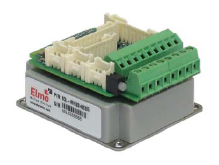
\includegraphics[width=0.82\textwidth]{latex_assets/image4.png}
\end{figure}

\begin{center}\zihao{5}图2.2 Solo Whistle数字伺服驱动器\end{center}

这款Solo Whistle数字伺服驱动器既可以作为一个独立的装置运行，也可作为多轴分布式网络系统中的一部分。Solo Whistle数字伺服驱动器可以工作在位置、速度和转矩等控制模式，能够对伺服电机进行高精度的控制，具有响应速度快、可靠性高、定位准确、运行平稳等优点，被广泛应用于各种工业自动化领域[8]。

\subsection{2.1.3 微控制器的选型}

微控制器是同轴驱动控制系统的进行算法分析和控制处理的主体，选型的合理性需要综合多方面进行考虑，比如恶劣的工业现场环境对可靠性和稳定性的要求，同轴驱动对数据传输的实时性要求和系统的低功耗性能等。

传统的8位和16位微处理器由于字长的限制，内核的运算速度和处理能力越发显得不足，特别是现场仪器仪表控制对智能化和多功能化的需求，8位和16位微处理器不够丰富的外设使的设计越发困难，而32位微处理器的出现，一定程度上解决了上述困境，并将成为今后设计的主流。

自2007年6月以来，意法半导体公司推出了多种系列的基于Cortex-M4内核的STM32微控制器。其中，STM32F4系列堪称全球最高性能的微控制器，根据应用场合的不同，可以选择STM32F4系列的不同型号的产品。

本课题选用ST公司开发的STM32F407作为微控制器，STM32F407是基于ARM Cortex-M4内核的32位闪存微控制器，STM32F4系列微控制器集成了FPU（Floating Point Unit，浮点运算单元）和单周期DSP（Digital Signal Processing，数字信号处理）指令，具有了处理数字信号的高速运算能力[9]。

STM32F4相对于STM32F1，主要优势包括：内核更为先进，片外资源丰富，外设功能增强，性能速度得到提高，功耗降低。

因此，选用的这款微控制器能显著提升控制算法的执行速度和代码效率，提升了算法的浮点运算处理速度和数字信号处理能力，满足了双电机同轴驱动控制系统对实时性、快速性和稳定性的要求。

\subsection{2.1.4 CAN总线高层协议的选择}

现场总线技术在工业生产领域应用广泛，其中CAN总线技术因为具有控制方式多样，可靠性、可操作性和实时性好，现场接线方式简单和成本较低等优点，被广泛应用于汽车产业和工业控制等领域。所以本课题一开始就考虑到运用CAN总线作为底层通信和控制网络，接下来需要进行CAN总线的高层协议的选择。

CAN总线协议对通信系统的物理层和数据链路层进行了规范，没有对应用层的具体实现加以规范，因此需要一种基于CAN总线的高层协议，对CAN报文中的11/29位标识符和8字节数据的用途加以规范[10]。

目前，在CAN总线的高层协议中，应用比较广泛的是CANopen和DeviceNet两种协议。首先DeviceNet主要应用于过程控制，CANopen主要应用于运动控制。特别地，CANopen具有针对伺服驱动设备的DSP402协议，因此主要考虑运用CANopen协议作为CAN总线的高层协议，另外在选用了Solo Whistle数字伺服驱动器后，通过阅读驱动器参考手册发现该数字伺服驱动器支持CANopen协议。采用CANopen协议也可以满足系统对速度、可靠性和抗干扰能力等要求，所以最终确定采用CANopen协议作为CAN高层协议。

\section{2.2 系统主要模块介绍}

\subsection{2.2.1 微控制器STM32F407特性简介}

意法半导体公司在2011年推出了基于Cortex-M4内核的STM32F4系列的微控制器，相比之前的STM32F1、STM32F2等系列的Cortex-M3产品，STM32F4最大的优势，就是集成了单周期的数字信号处理指令和浮点运算单元，同时，STM32F4的主频提高到168Mhz，比STM32F1主频的72Mhz提升达到2倍以上，这使得STM32F4尤其适用于需要浮点运算或数字信号处理的场合，因此具有非常广阔的应用前景。

丰富的外设资源和高效的处理速度使得STM32F407微控制器能够适用于本课题的双电机同轴驱动控制系统中，保证了系统对实时性、快速性和稳定性的要求。STM32F4系列目前拥诸多系列和产品型号，这些型号之间兼容性十分完备，便于移植和升级。

\subsection{2.2.2 Solo Whistle数字伺服驱动器简介}

以色列Elmo的智能SimplIQ驱动器可以完成工业现场很多复杂的控制任务，而采用的Solo Whistle数字伺服驱动器是SimplIQ产品线的一部分，应用Elmo的Metronome运动控制语言，完全可编程。

\subsection{2.2.3 直流无刷电机参数介绍}

伺服电机是构成伺服系统的关键部件之一，作为系统的执行部件，其质量好坏直接影响到系统的诸多重要性能。考虑到直流无刷电机具有良好的调速性能，控制电路简单，低速性能好，没有励磁损耗，同时利用的电子换相具有故障率低、性能可靠和没有磨损的特点。基于以上几点，本课题选用两个参数相同的直流无刷电机BMSCA50，其主要参数如表2.1所示。

\begin{center}\zihao{5}表2.1 BMSCA50直流无刷电机主要参数\end{center}

\begin{table}[htbp]
\centering
\zihao{5}
\renewcommand{\arraystretch}{1.25}
\begin{tabularx}{0.88\textwidth}{|>{\centering\arraybackslash}p{0.28\textwidth}|X|}
\hline
参数 & 值 \\
\hline
电压 & 24V DC \\
\hline
额定功率 & 55W \\
\hline
额定电流 & 3A \\
\hline
额定转矩 & 0.16N.m \\
\hline
额定转速 & 3300rpm \\
\hline
电机级数 & 4 \\
\hline
减速比 & 1/55 \\
\hline
输出转速 & 60rpm \\
\hline
输出转矩 & 6.4N.m \\
\hline
编码器脉冲数 & 1000P/R \\
\hline
电机齿轮与负载轴速比 & 4/5 \\
\hline
\end{tabularx}
\end{table}

\section{2.3 本章小结}

本章主要介绍了双电机同轴驱动控制系统的总体方案设计，包括控制系统的总体电器结构，再到重要组成部分伺服驱动器、微控制器和CAN总线高层协议的选择方案论证，最后对主要模块的一些参数作了介绍和说明。

\chapter{第三章 同轴驱动控制系统硬件设计}

同轴驱动控制系统的核心板以STM32F407芯片为主控芯片，主要负责控制算法的实现、对数字伺服驱动器指令的发送和数据的监测以及数据与上位机的交互等，通过与外围各个模块的电气连接，最终实现所需功能和指标。核心板主要部分的总体结构硬件框图如图3.1所示。

\section{3.1 STM32F407最小系统板设计}

\subsection{3.1.1 芯片外围电路}

XXX电路如图3.3所示。…………。

% Unsupported Word vector image omitted: latex_assets/image5.emf
\begin{center}
\fbox{\parbox{0.75\textwidth}{Word vector image placeholder: image5.emf}}
\end{center}

\begin{center}\zihao{5}图3.3 主控板下载电路\end{center}

\subsection{3.1.2 电源电路}

\subsection{3.1.3 时钟电路}

\subsection{3.1.4 复位电路与启动模式设置}

\section{3.2 通信模块设计}

\subsection{3.2.1 CAN通信电路}

\subsection{3.2.2 串口通信电路}

\subsection{3.2.3 NFR24L01通信接口电路}

\section{3.3 OLED显示模块接口设计}

\section{3.4 调试电路设计}

\section{3.5 外围模块电路设计}

\subsection{3.5.1 按键电路和LED电路}

\subsection{3.5.2 RTC实时时钟供电电路}

\subsection{3.5.3 引出IO和供电管脚电路}

\section{3.6 PCB设计}

\section{3.7 本章小结}

本章主要介绍了本课题中的同轴驱动控制系统硬件设计，在确定引脚分配的基础上，首先设计了STM32F407最小系统板的原理图，然后按照所需的各个模块，分别设计了通信模块，调试电路，外围模块电路，最后完成整个系统核心板的PCB布局和连线，并总结了PCB设计时遇到的问题和注意事项。核心板的制作完成，为后续的软件设计和算法研究提供了硬件支持。

\chapter{第四章 同轴驱动控制系统算法研究及MATLAB仿真}

双电机同轴驱动系统较单电机驱动系统复杂，两个电机共同驱动同一负载，涉及两台电机的同步问题，且对负载速度和位置进行精确控制。同轴驱动系统目的是是增大输出功率或消除传动齿隙非线性对控制精度影响，因此需要相应的控制算法消除齿隙，达到对负载的精确控制，本章将重点研究双电机同轴驱动控制算法和消隙控制算法。

\section{4.1 双电机同轴驱动控制算法}

双电机同轴驱动不同于普通双电机柔性同步控制系统，双电机共同驱动同一负载，属于刚性同步控制范畴。理想双电机驱动系统具有完全相同的各项参数，则输入相同的指令时，输出速度保持一致，但电机制造、编码器反馈、传动链、元器件等存在差异，两套电机驱动系统即使在相同的速度指令下，输出速度存在差异，导致两个电机的速度不同步，造成功率的损耗，影响系统的正常使用[21]。

针对这一问题，研究人员研究多种同步控制算法，如直接差速负反馈法I和直接差速负反馈法II，主从差速负反馈控制法和间接差速负反馈控制法等[22]。这些算法具备能够在一定程度上解决双电机速度同步问题，但也存在控制系统复杂等不足。

本课题采用单速度环实现双电机同轴驱动控制，将两个电机的速度反馈信号取平均值作为唯一的速度反馈值，一方面相当于对速度值进行了滤波，另一方面保证了整个系统只有一个速度反馈，可以使两个电机的转速都朝着所取的平均值靠近，从而迅速跟踪给定的速度信号，并实现两个电机的转速相等，保证成两个电机的输出转矩达到均衡，使得系统趋于稳定[23]。

\section{4.2 双电机同轴驱动消隙控制算法}

\section{4.3 双电机同轴驱动控制回路设计}

\subsection{4.3.1 电流环设计}

\subsection{4.3.2 速度环设计}

速度环原理框图如图4.3所示，速度环增大电机的调速范围，改善动态特性和抗干扰能力，为实现双电机同轴驱动控制，常采用双闭环的控制方式，即速度环、电

流环双闭环控制，双电机双闭环控制系统结构框图如图4.4所示[28]。速度环的反馈采用的是4.1小节中提到的速度均衡算法，即采用双电机的速度反馈值的均值，通过对两个电机的转速值求平均，作为速度反馈值。图4.4中，ASR为速度环调节器，由于可以将数字伺服驱动器设置成转矩控制模式，因此ACR1和ACR2两个电流环调节器和两个功率驱动单元组成的电流环包含在数字伺服驱动器中。

\subsection{4.3.3 位置环设计}

\subsection{4.3.4 三闭环综合设计}

\section{4.4 PID控制算法设计}

在设计电流环、速度环和位置环的过程中，还需要考虑的是电流调节器、速度调节器和位置调节器的控制算法，在工业控制中，常采用PID控制算法。本课题的控制器采用的是STM32F407VET6，控制上属于离散系统，因此需要采用数字PID控制算法代替模拟PID算法。

\subsection{4.4.1 数字PID控制算法研究}

PID控制就是按偏差的比例、积分和微分对系统进行控制的一种方法，在连续系统中应用广泛，随着计算机控制的不断发展和数字离散系统的大量使用，使得数字PID算法逐渐代替了模拟PID算法，成为计算机工控领域应用最广泛的一种算法[29]。

当采样周期足够小时，可以采取数值逼近的方法，将模拟 PID 离散化变为差分方程，如公式(4-1)至(4-4)所示：

（4-1）

（4-2）

（4-3）

（4-4）

式中：T表示采样周期，k表示采样序号。用这种近似方法，可得到以下两种标准的数字PID控制算法。

\noindent （1）数字PID位置型控制算法\\

数字PID位置型控制算法如公式（4-5）所示：

（4-5）

\noindent （2）数字PID增量型控制算法\\

由公式（4-5）可以看出，位置型控制算法需要累加所有偏差e(j)，会占用较多的存储单元，使用不方便，可对公式（4-5）进行如下改进。

根据公式（4-5）表示出u(k-1)的表达式，即：

（4-6）

\subsection{4.4.2 控制系统数字PID控制器设计}

\section{4.5 控制算法仿真}

\subsection{4.5.1电机的Simulink闭环控制模型}

\subsection{4.5.2 双电机同轴驱动双速度环仿真}

\subsection{4.5.3 双电机同轴驱动单速度环仿真}

\subsection{4.5.4 双电机同轴驱动消隙控制算法仿真}

\subsection{4.5.5 速度PI控制器仿真实验}

MATLAB中利用Simulink搭建的双电机双闭环控制系统的仿真模型如图4.18所示。

\begin{figure}[htbp]
\centering
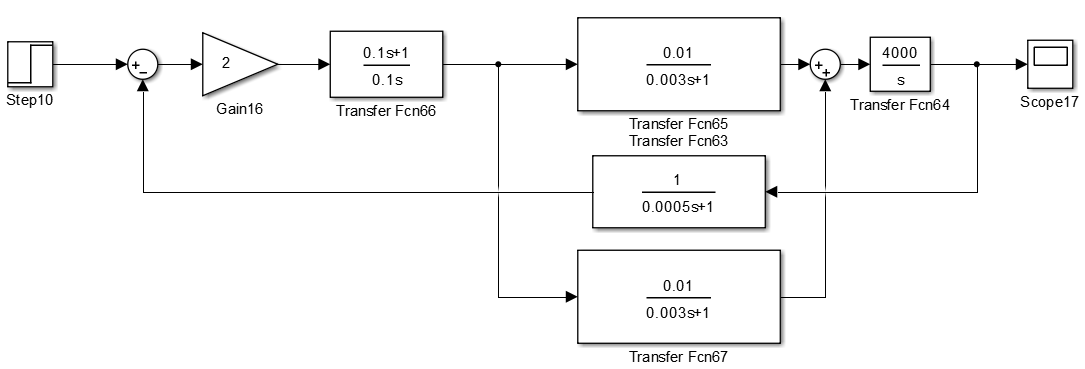
\includegraphics[width=0.82\textwidth]{latex_assets/image12.png}
\end{figure}

\begin{center}\zihao{5}图4.18 双电机双闭环控制系统的Simulink仿真模型\end{center}

由Simulink搭建的仿真模型中，阶跃信号在T=0.1秒时，输出阶跃波形阶跃的幅值为50度/秒。速度调节器一般均采用的是PI调节器。速度反馈采取的是速度均衡算法，没有加消隙控制算法中所需的偏置力矩。

因为电流环已经包含在伺服驱动器内部，所以无法对电流环进行控制，实际应用中只能调节速度PI调节器，改变比例和积分常数。当Kp=2，Ti=0.9；Kp=4，Ti=0.9；Kp=2，Ti=0.1；Kp=4，Ti=0.1时双电机双闭环速度输出波形分别如图4.19\textasciitilde{}图4.21所示。

% Unsupported Word vector image omitted: latex_assets/image13.emf
\begin{center}
\fbox{\parbox{0.75\textwidth}{Word vector image placeholder: image13.emf}}
\end{center}
% Unsupported Word vector image omitted: latex_assets/image14.emf
\begin{center}
\fbox{\parbox{0.75\textwidth}{Word vector image placeholder: image14.emf}}
\end{center}

\begin{center}\zihao{5}图4.19 速度输出波形（Kp=2，Ti=0.9） 图4.20 速度输出波形（Kp=4，Ti=0.9）\end{center}

% Unsupported Word vector image omitted: latex_assets/image15.emf
\begin{center}
\fbox{\parbox{0.75\textwidth}{Word vector image placeholder: image15.emf}}
\end{center}
% Unsupported Word vector image omitted: latex_assets/image16.emf
\begin{center}
\fbox{\parbox{0.75\textwidth}{Word vector image placeholder: image16.emf}}
\end{center}

\begin{center}\zihao{5}图4.21 速度输出波形（Kp=2，Ti=0.1） 图4.21 速度输出波形（Kp=4，Ti=0.1）\end{center}

由上述仿真实验，对比分析可得如下两个结论：

\noindent （1）当积分常数不变时，比例常数由2提高到4，速度输出波形的调节时间减小，但是超调量增加，可能会造成系统的不稳定。\\

\noindent （2）当比例常数不变时，积分时间常数由0.9减小为0.1，即积分常数增大，导致速度输出波形的调节时间减小，但是超调量增加，也会造成系统的不稳定。\\

\section{4.6 本章小结}

本章主要介绍了双电机同轴驱动控制系统中控制算法，包括双电机同步所需的速度均衡控制算法和消隙所需的偏置力矩控制算法，并进行了同轴驱动控制系统的三闭环设计，最后对调节器的PID增量型控制算法做了简要说明。在此基础上进行了单电机速度、电流双闭环的模型分析，引入到双电机速度、电流双闭环的模型，完成了双电机双闭环系统方框图后，在Simulink环境下，完成了双电机双闭环仿真模型的简化和搭建，并对速度PI控制器和双电机同步算法进行了仿真分析，得出了相应的结论，为后续的实物测试应用奠定了基础。

\chapter{第五章 同轴驱动控制系统软件设计}

以STM32F407为核心的核心板主要完成位置环、速度环的功能，消隙所需的偏置力矩给定和速度均衡控制功能也在控制器中实现。微控制器的得到的位置信号偏差，通过PI控制器，作为位置环的输入；微控制器得到的速度信号偏差，通过P或PI控制器，作为电流环的输入，进行转矩给定，实现对两个电机的控制，驱动同一负载。另外由于该控制系统的通信网络是基于CAN总线和CANopen高级协议的，因此还需要实现总线和底层协议的编写，由于进度原因，下面的软件设计仅完成速度环和电流环的软件部分编写。

该伺服控制器的软件设计采用模块化设计方法，首先将各个不同的模块的底层进行封装测试处理，并放在每个模块对应的C语言文件.c和.h里，对外留出接口函数便于调用，这样每个模块的关联和耦合度会降到最低，便于程序的移植和修改。

同轴驱动控制系统软件部分主要包含三大模块，一是主程序，二是中断服务程序，三是参数显示程序和串口通信程序，控制算法等核心程序都在中断服务程序中进行编写。

\section{5.1 主程序设计}

\subsection{5.1.1 CAN 模块初始化流程}

\subsection{5.1.2 伺服驱动器初始化}

\section{5.2 子程序设计}

\subsection{5.2.1 CAN中断服务程序}

根据CAN过滤器的配置，接受来自伺服驱动器的所有报文，CAN中断服务程序最主要的作用是从接收邮箱中读出报文，利用RxMessage.StdId的不同，用switch(RxMessage.StdId)语句对所收报文进行分类，判断得出是哪个伺服驱动器发送的速度或转矩信息，并存入相应的变量中，相当于有了闭环反馈信号。当邮箱接收到数据时，必须要在中断内调用CAN\_Receive函数读取接收FIFO的内容，因为只有这样才能清除该FIFO的接收中断标志。CAN中断接收流程图如图5.4所示。

\subsection{5.2.2 定时器中断服务程序}

\section{5.3 参数显示程序和串口通信程序}

在主程序进入了循环后，循环中主要完成按键的扫描和OLED数据实时更新，参数显示程序通过编写OLED显示界面，实时显示所需电机速度参数反馈和电机输出转矩数值大小，方便进行观察和调试。

串口通信程序在进入了循环之前，提示程序准备进入了循环，程序编写如下：

printf("\textbackslash{}r\textbackslash{}n 这是双电机同轴驱动控制系统实验\textbackslash{}r\textbackslash{}n");

printf("\textbackslash{}r\textbackslash{}n 1.按下S3键，会发送一次数据\textbackslash{}r\textbackslash{}n");

printf("\textbackslash{}r\textbackslash{}n 2.收到会打印到串口 \textbackslash{}r\textbackslash{}n");

printf("\textbackslash{}r\textbackslash{}n3.本例中的CAN波特率为500KBps，1MBps为STM32的CAN最高速率\textbackslash{}r\textbackslash{}n");

实际监测效果如图5.8所示。

\begin{figure}[htbp]
\centering
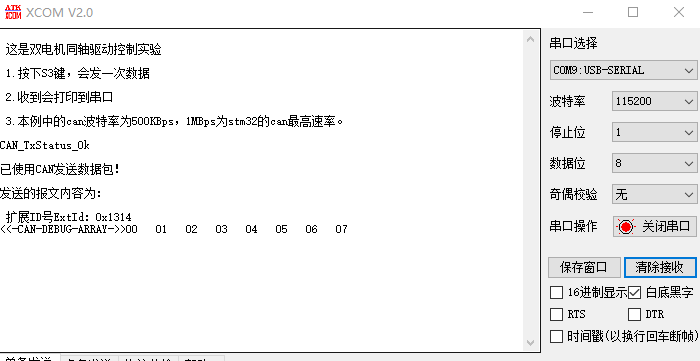
\includegraphics[width=0.82\textwidth]{latex_assets/image17.png}
\end{figure}

\begin{center}\zihao{5}图5.8 串口实际监测效果\end{center}

而OLED显示界面主要显示了TorL 、TorR、VelL和VelR值，分别表示左电机转矩、右电机转矩、左电机速度和左电机速度。显示界面程序编写如下：

OLED\_Show\_FONT\_6x8(4, 1, "TorL:");

OLED\_Show\_FONT\_6x8(5, 1, " TorR:");

LCD\_write\_Torque\_data(4, 6, Current\_left\_Torque);

LCD\_write\_Torque\_data(5, 6, Current\_right\_Torque);

OLED\_Show\_FONT\_6x8(6, 1, "VelL:");

OLED\_Show\_FONT\_6x8(7, 1, "VelR:");

LCD\_write\_Velocity\_data(6, 6, Current\_left\_Velocity);

LCD\_write\_Velocity\_data(7, 6, Current\_right\_Velocity);

\section{5.4 本章小结}

本章详细介绍了双电机同轴驱动控制系统软件的总体设计思想和代码实现，以STM32F407核心板为硬件基础，综合设计出按键电路驱动程序、LED电路驱动程序、OLED显示电路底层驱动程序，在研究了CAN总线和CANopen高级协议的基础上，通读了针对Elmo电机控制的CANopen DS301和DSP402协议实施指南，完成了CAN底层电路驱动程序和CANopen高级协议DS301和DSP402的设计，为后面的算法实现提供了底层函数接口和支持。

控制系统基本算法主要在中断服务程序中编写，实现了速度环，电流环的闭环控制，完成了消隙功能和双电机速度同步功能。同样为了调试，设计了参数显示程序和串口通信程序。

\chapter{第六章 系统调试、结果与成本分析}

\section{6.1 系统调试与分析}

在设计完同轴驱动控制系统的软硬件和算法之后，最后需要进行整个系统的联调，保证能够满足系统所需的性能指标。

\subsection{6.1.1 核心板硬件调试}

核心板的硬件设计，是双电机同步控制算法、消隙控制等软件实现的基础，因此在PCB制板完成之后要确保核心板上各个模块调试的正确，保证基于CANopen协议的CAN通信正常。

\noindent （1）测试实验\\

在CAN通信的回环模式下，输出端的所有内容都直接传输到输入端，输出端的内容同时也会被传输到总线上，可使用总线监测发送内容。因此可以设置成回环模式可以进行自检，以检验CAN通信模块的软硬件设计的正确性。这里将数据通过串口发送到上位机电脑上，并在串口调试助手上显示出来，测试验证了核心板CAN通信模块的软硬件设计的正确性，如图6.1所示。

\begin{figure}[htbp]
\centering
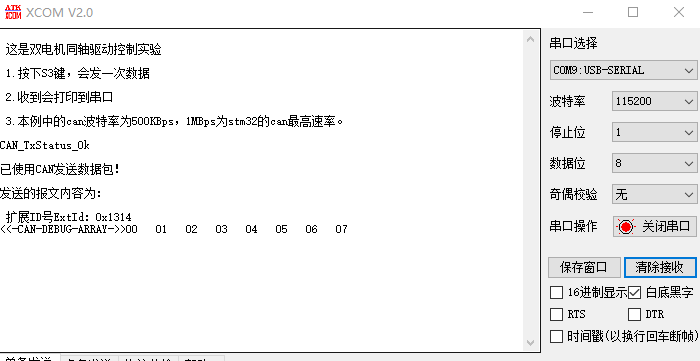
\includegraphics[width=0.82\textwidth]{latex_assets/image17.png}
\end{figure}

\begin{center}\zihao{5}图6.1 CAN通信模块测试\end{center}

\noindent （2）存在的问题\\

在检查设计的双CAN模块时，发现两个CAN模块的引脚都连在了CAN1控制器的引脚（PD0、PD1和PA11、PA12）上，这样就不能实现双CAN收发数据，因此需要将其中一个CAN的信号引脚改接到PB5、PB6上，由CAN2控制器进行控制。

\subsection{6.1.2 电机控制调试}

\section{6.2 数据结果记录与分析}

\subsection{6.2.1 比例调节器控制实验}

\noindent （1）单电机双闭环测试\\

将伺服驱动器的控制模式设置成转矩模式，对单个电机进行速度、电流双闭环测试，速度调节器采用比例控制方式。当单个电机速度给定值为100,000（这里的100,000表示脉冲数，速度给定55,000时，电机外齿轮转一圈需要4秒），Kp=0.003 和Kp=0.03时，测得的实验波形分别如图6.9和图6.10所示。

\begin{figure}[htbp]
\centering
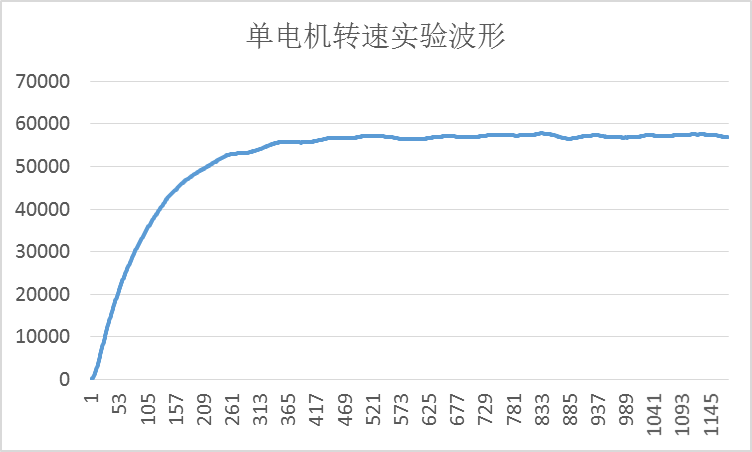
\includegraphics[width=0.82\textwidth]{latex_assets/image18.png}
\end{figure}
\begin{figure}[htbp]
\centering
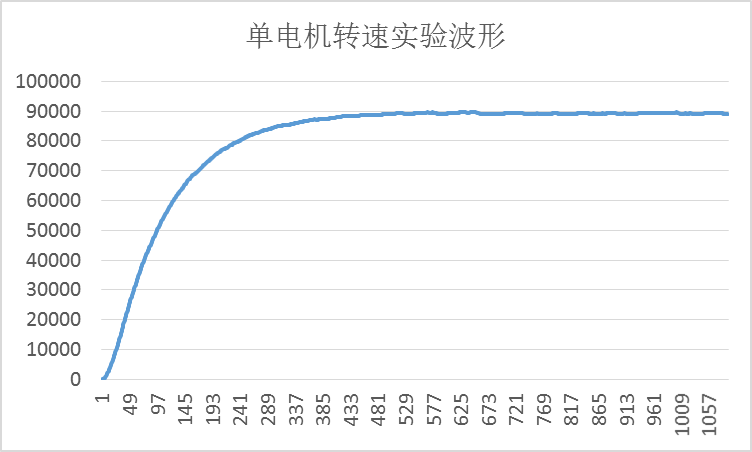
\includegraphics[width=0.82\textwidth]{latex_assets/image19.png}
\end{figure}

\begin{center}\zihao{5}图6.9 单电机转速波形（Kp=0.003） 图6.10 单电机转速波形（Kp=0.03）\end{center}

经过上述四组波形的测试结果分析：通过增大比例系数，可以加快系统的响应速度，但是比例系数过大时，会引起系统的轻微震荡。由于只存在比例调节，系统总是存在静差，但是随着比例系数的增大，静差会减小，但是不能消除。

\subsection{6.2.2 比例积分调节器控制实验}

上述实验是在比例调节器的作用下进行的控制实验，所以系统存在静差，相对于伺服驱动器在低速时对电机的控制效果来说，比例调节器的控制效果并不是十分理想，因此有必要引入积分环节，采用比例积分调节器。

在保证系统不发生震荡的情况下，在低速时对双电机进行了由比例积分调节器控制的速度、电流双闭环测试实验，当速度给定值为1,000时，Kp=0.012，Ti=100时，测得的转矩波形和速度波形分别如图6.17和6.18所示。

\begin{figure}[htbp]
\centering
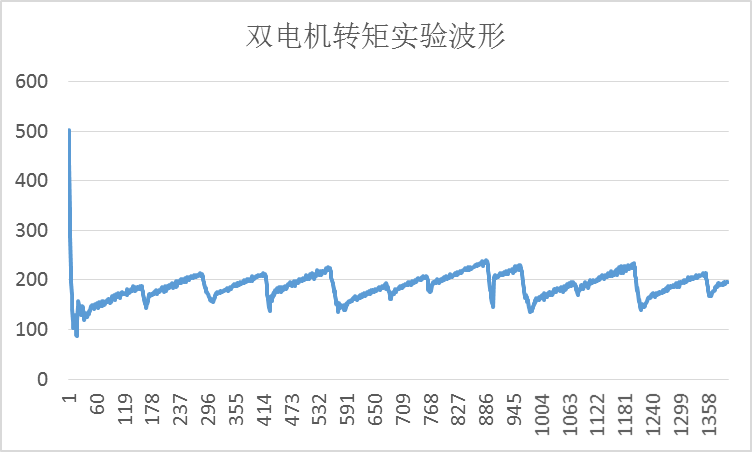
\includegraphics[width=0.82\textwidth]{latex_assets/image20.png}
\end{figure}
\begin{figure}[htbp]
\centering
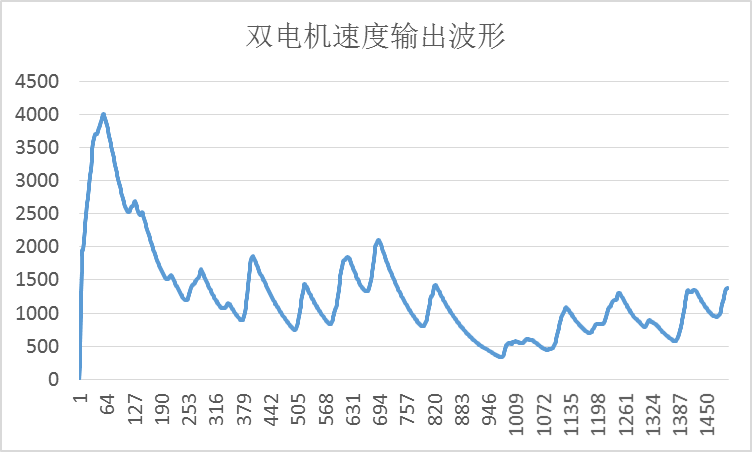
\includegraphics[width=0.82\textwidth]{latex_assets/image21.png}
\end{figure}

\begin{center}\zihao{5}图6.17 双电机转矩实验波形 图6.18 双电机速度输出波形\end{center}

由测得的转矩波形分析可知，系统速度有差时，比例和积分均产生作用，当积分到给定值时，系统速度没有偏差，因此转矩迅速回落，因此转矩波形呈现出周期性的波浪形。再观察速度输出波形，发现刚开始速度有一个很大的超调量，这是因为电机刚开始转动时，需要克服自身较大的摩擦转矩，随后速度回落并在1,000附近发生较为明显的波动，相比较图6.15的速度波形，比例积分调节器控制效果并不是十分理想，但是又比纯比例调节器的控制效果好很多，将调速范围扩大到了1,000值20,000。

\subsection{6.2.3 偏置力矩作用对比实验}

\subsection{6.2.4 双电机同步控制中的滤波实验}

\section{6.3 系统成本分析}

注意：课题性质为工程设计类的毕业设计，需要有系统设计成本分析。能够运用工程管理与经济决策方法分析影响系统设计成本的因素。

\section{6.4 本章小结}

本章主要记录了本次实验的主要过程，从核心板的硬件调试，到通过CAN总线对电机进行控制测试，在这些实验中发现了不少问题，查找并提出了适当的解决办法，逐步实现了双电机的双闭环控制。在实现双电机的双闭环控制的过程中，先记录单电机实验数据，研究了单电机速度控制的波形图，分析了比例、比例积分速度控制器的不同点，然后过渡到双电机速度控制，对比分析了双电机同步控制算法和消隙控制算法对实验波形的影响，得出了相关结论。

\chapter{第七章 总结与展望}

\section{7.1 全文总结}

本课题选自现代工业控制中的大功率负载驱动任务，主要实现了一种基于CANopen协议的双电机同轴驱动控制系统。本论文首先进行总体方案的设计，包括系统总体电气结构的设计，到伺服驱动器、微控制器的选型和通讯方式的选择，在经过不同方案对比论证以后，选出了符合本课题基本要求的设计。

本课题属于一个完整的综合工控课题，涉及面比较广泛，本论文先介绍了该驱动控制系统的数据通讯的基本方式CAN通信和CANopen高级协议，论文的重点部分放在控制系统的硬件设计、软件设计和同轴驱动时所涉及到的控制算法上。硬件设计的完成，为双电机同步控制和消隙控制算法提供了硬件基础。在经过算法的Simulink仿真之后应用到实际的调试中去。最后，设计了系统软件，通过软件的方式实现了同步控制功能和消隙控制，由最终的实物测试结果来看，基本达到了驱动任务的性能指标要求。

论文的特色与创新有：

\noindent （1）全数字化控制。采用数字化、模块化的设计理念，应用CANopen高级协议完成系统控制，运用数字PID增量型控制算法，配合通用的数字伺服驱动器，提高了控制精度，增强了抗干扰能力，简化了系统设计，系统重构性好、易于扩展和移植。\\

\noindent （2）系统实时性强。系统核心板以STM32F407为核心，该控制器集成DSP和FPU指令，可以提升内部环路的浮点运算速度和数字信号处理能力。采用双CAN控制器，使得单个CAN总线数据负荷降低，合理规划通讯时序，定时器中断服务周期降至5ms以内，保证通讯的实时性。\\

\noindent （3）同轴驱动控制算法。本课题提出了双电机同步控制算法和消隙控制算法，并在此基础上又引入了多闭环控制方式，采用的数字PI控制方式，保证了系统的动态性能和稳态要求。\\

\section{7.2 研究展望}

在本课题的设计中，基本达到了双电机同轴驱动任务的性能指标要求。但是由于实验条件和时间的限制，还存在着诸多不足和部分功能未能实现，主要包括：

\noindent （1）双电机同轴驱动的实际调试时，仅采用了速度、电流双闭环控制算法，位置环还没有加上，因此负载的调速范围整体偏小，位置控制精度偏低。\\

\noindent （2）实际调试中实现了双电机同步控制和消隙控制算法，但是同步控制方法还需要继续完善，消隙控制只加上了固定的偏置力矩，这只是一种很粗略的控制方式，还有待改进，比如加上动态的偏置力矩。\\

\noindent （3）控制系统的算法和模型仿真时并未考虑到摩擦力等因素的影响，因此后续的工作会考虑到摩擦因素，并进行相关研究，使系统的快速性和稳定性通过调整参数和控制算法进一步提高。\\

\chapter{致 谢}

致谢是作者向在自己学习、生活、特别是毕业设计（论文）完成过程中帮助过自己的人表达感谢，每位同学根据自己的实际情况进行描述。

xxx

二二四年五月 于南京

\chapter{参考文献}

张磊. 基于CAN总线的全数字交流伺服系统的研究与开发[D]. 山东大学, 2005.

正军. 现场总线及其应用技术[M]. 机械工业出版社, 2005.

许万. 基于实时以太网的多轴运动控制系统研究[D]. 武汉: 华中科技大学, 2009.

杨中群. 多电机同步控制系统的研究与设计[D]. 武汉理工大学, 2013.

黄磊. 基于双电机驱动系统的间隙消除技术研究[D]. 武汉: 华中科技大学, 2007.

刘然, 孙建忠, 罗亚琴, 等. 基于环形耦合策略的多电机同步控制研究[J]. 控制与决策, 2011, 26(6): 957-960.

贺安超, 刘卫国, 马珊. 基于CAN总线的多电机嵌入式监控系统设计[J]. 计算机测量与控制, 2011, 19(7): 1605-1607.

STMicroelectronics. RM0090 Reference Manual for STM32F405/415, STM32F407/417, STM32F427/437 and STM32F429/439 advanced ARM®-based 32-bit MCUs. [EB/OL], [2015-10-20]. http://www.st.com.

万鹏飞, 王莉. 基于模糊 PID 控制的多电机同步控制研究[J]. 仪器仪表用户, 2009, 16(1): 21-23.

王晓辉. 基于 CAN 总线的智能数据采集模块的设计与实现[D]. 河南科技大学, 2012.

丁勇, 张吉堂. 基于CAN总线的伺服电机正反转同步控制[J]. 机床与液压, 2014, 42(4): 95-97.

孙铁兵, 鞠宁. CAN总线及其高层协议[J]. 微处理机, 2006, 27(1): 24-26.

徐杰, 金海, 鲁文其. 基于CAN总线通信的双电机速度联动控制系统设计[J]. 浙江理工大学学报, 2015, 33(2): 209-213.

马成才. 基于CANopen协议的交流伺服驱动器从站研究[D]. 南京航空航天大学, 2012.

Kang M J, Park J H, Kim J H, et al. A disturbance observer design for backlash compensation[J]. International Journal of Control, Automation and Systems, 2011, 9(4): 742-749.

王玮, 史伟民, 鲁文其, 等. 基于CAN总线的多轴位置伺服联动系统设计与性能分析[J]. 浙江理工大学学报, 2015, 33(1): 95-99.

张捍东, 徐龙, 岑豫皖. CANopen协议及在 ARM 控制多电机驱动器系统中的应用与设计[J]. 自动化与仪器仪表, 2011 (2): 40-43.

陈锐, 张鑫, 孙景龙. 基于STM32F4xx的CAN总线设计与应用[J]. 黑龙江科技信息, 2013 (28): 163-163.

Zhang P, Zhang J H, He D S, et al. Based on adjacent cross-coupling of multi-motor synchronous drive[C]. Advanced Materials Research. 2011, 201: 1093-1097.

\chapter{附录A：硬件设计原理图}

\chapter{附录B：硬件设计PCB图}

PCB板顶层图

\begin{figure}[htbp]
\centering
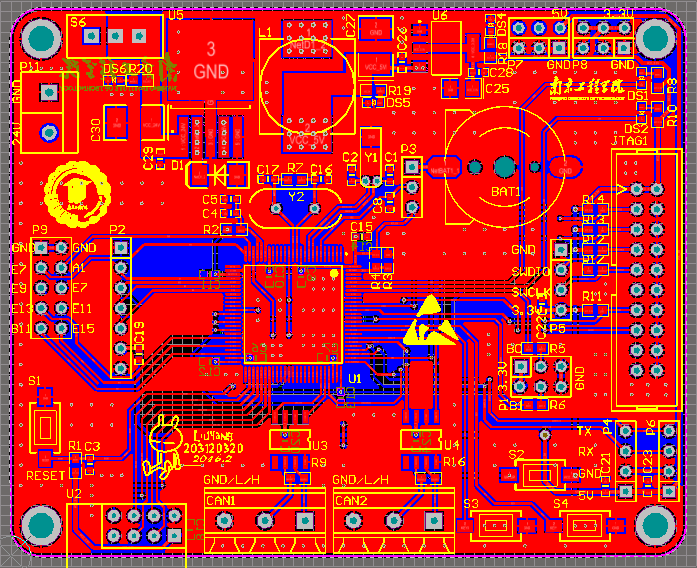
\includegraphics[width=0.82\textwidth]{latex_assets/image22.png}
\end{figure}

PCB板底层图

\begin{figure}[htbp]
\centering
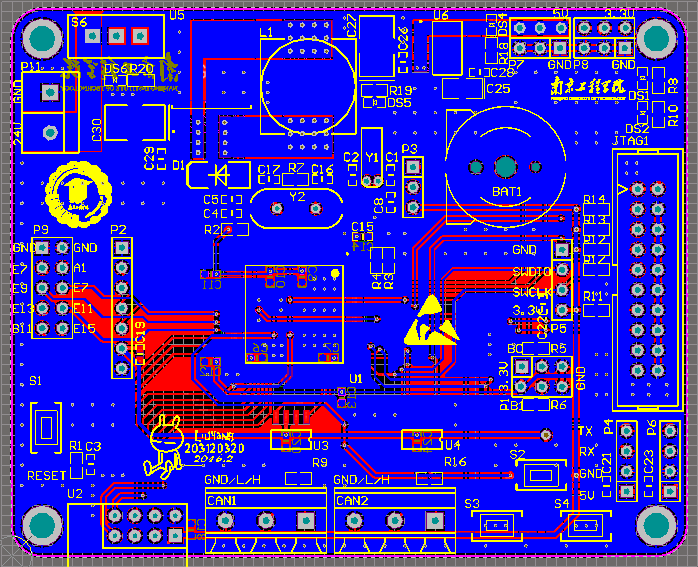
\includegraphics[width=0.82\textwidth]{latex_assets/image23.png}
\end{figure}

\chapter{附录C：PCB硬件实物图}

\begin{figure}[htbp]
\centering
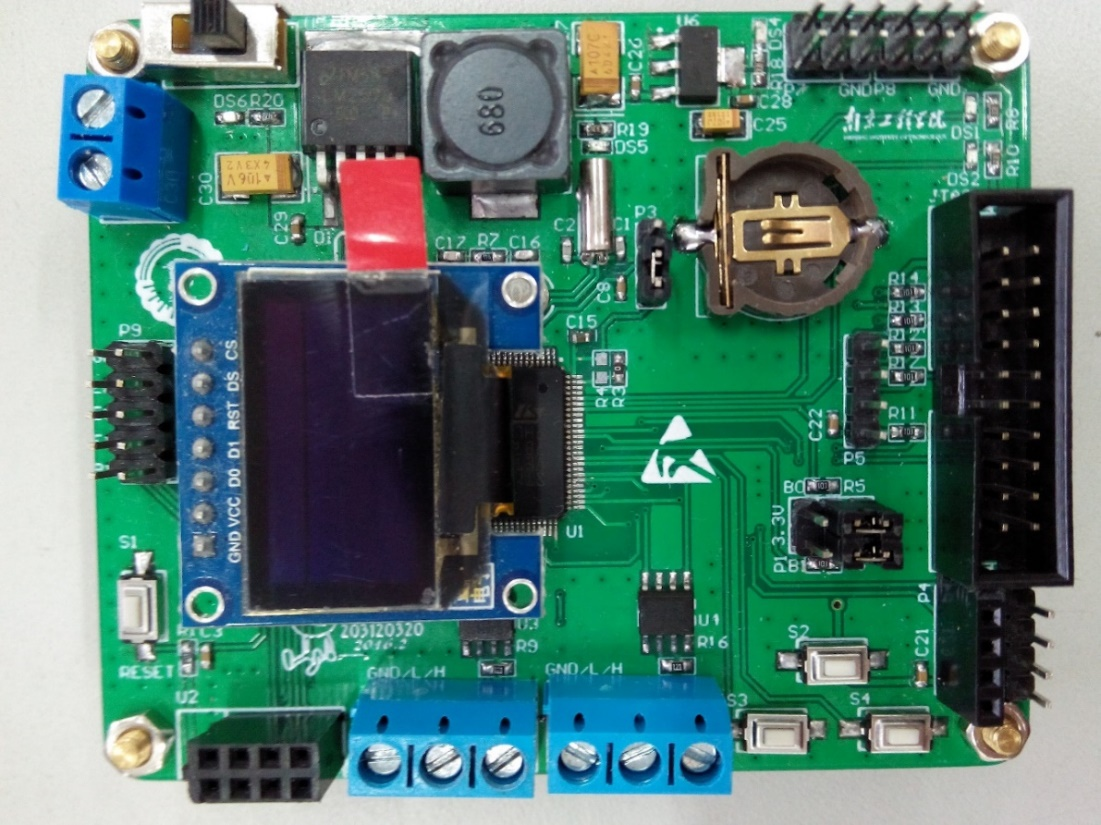
\includegraphics[width=0.82\textwidth]{latex_assets/image24.jpeg}
\end{figure}

核心板正面实物图

\begin{figure}[htbp]
\centering
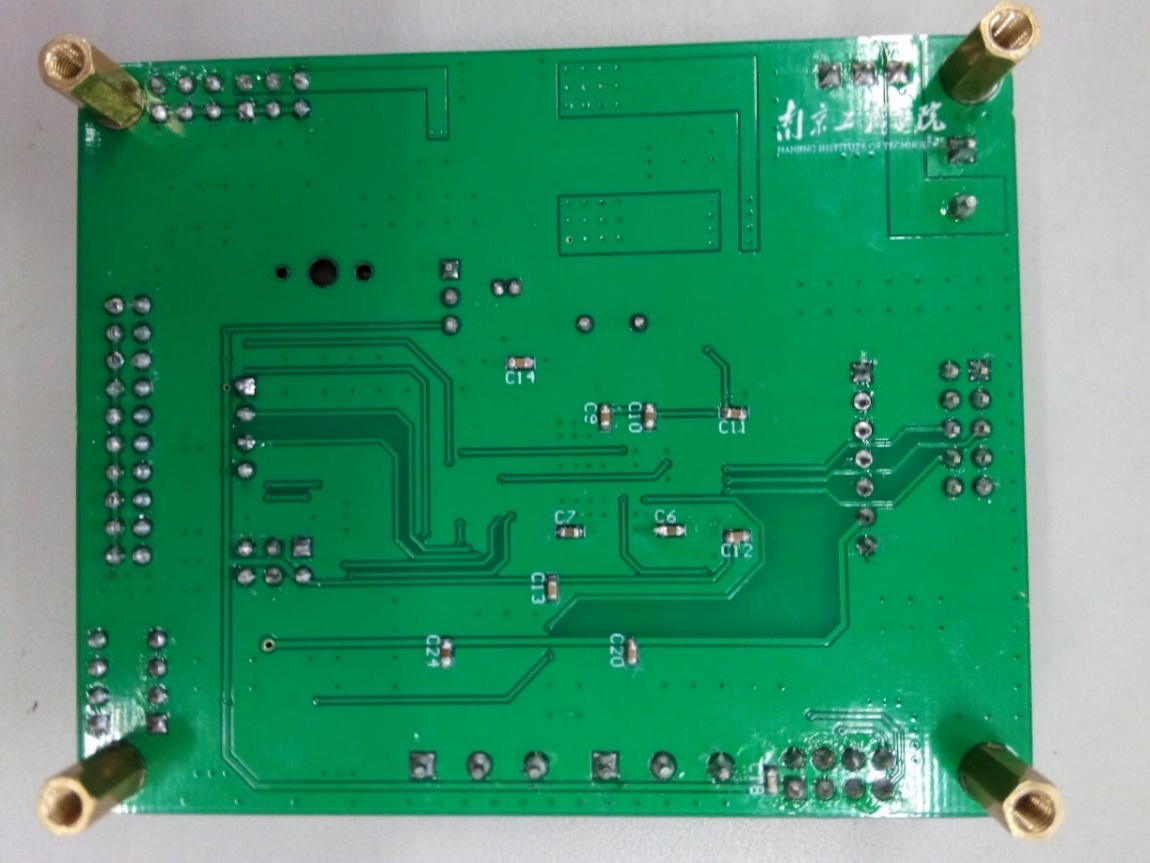
\includegraphics[width=0.82\textwidth]{latex_assets/image25.jpeg}
\end{figure}

核心板背面实物图

\chapter{附录D：主要程序清单}

1. 主程序

int main(void)

\{

delay\_init(168);

LED\_GPIO\_Config();

Key\_GPIO\_Config();

Debug\_USART\_Config();

printf("\textbackslash{}r\textbackslash{}n 这是双电机同轴驱动控制系统实验\textbackslash{}r\textbackslash{}n");

printf("\textbackslash{}r\textbackslash{}n 1.按下S3键，会发送一次数据\textbackslash{}r\textbackslash{}n");

printf("\textbackslash{}r\textbackslash{}n 2.收到会打印到串口 \textbackslash{}r\textbackslash{}n");

printf("\textbackslash{}r\textbackslash{}n3.本例中的CAN波特率为500KBps，1MBps为STM32的CAN最高速率\textbackslash{}r\textbackslash{}n");

LED1(ON);

delay\_ms(500);

LED1(OFF)；

Drive\_PDO\_Init(Drive\_left\_ID,Drive\_right\_ID);

delay\_ms(100);

SetDriveMode(Drive\_left\_ID, Torque\_profiled\_mode);//Profiled\_velocity\_mode Torque\_profiled\_mode

delay\_ms(100);

SetDriveMode(Drive\_right\_ID, Torque\_profiled\_mode);

delay\_ms(100);

EnableDrive(Drive\_left\_ID,1);

delay\_ms(100);

EnableDrive(Drive\_right\_ID,1);

delay\_ms(100);

while(1)

\{

\}

南京工程学院自动化学院

《本科毕业设计（论文）》撰写要求

本科毕业设计（论文）由“中文封面”、“英文封面”、“中文摘要”、“英文摘要”、“目录”、“绪论”、“正文”、“结论”、“致谢”、“参考文献”、“附录”等几部分组成。对本科毕业设计（论文）的撰写内容及格式要求如下。

1、内容要求

【特别注意：提供的模板不是完整的论文，只是总体框架，各部分内容均不完整，请勿简单参照模板现有篇幅完成论文！】

本科毕业设计（论文）应语言流畅、文字精炼、内容正确、条理分明、结构严谨、项目齐全；方案的分析与论证，要观点鲜明、过程清晰、结论正确；资料的查阅与引用，要全面客观、规范完整。图表和符号的应用，要规范、正确、清楚。

\noindent （1）中英文封面\\

中英文封面要信息完整、正确。

英文封面教师职称：Professor、Associate Professor、Lecturer、Professor of Engineering。

\noindent （2）中英文摘要\\

中文摘要应以第三人称陈述课题研究内容，主要包括研究目的、研究方法、研究结果和研究结论。摘要中一般不用图、表、计算机程序，不用非公知公用的符号、术语和非法定的计量单位。中文摘要300\textasciitilde{}500字左右。

英文摘要应与“中文摘要”对应，以第三人称陈述课题研究内容，用现在时态，强调过去已完成的工作时可采用过去时和现在完成时，尽可能采用被动语态。英文摘要250个左右实词。

\noindent\textbf{关键词是从论文中选取出来用以表示全文主题内容的术语或单词。关键词3-5个，分号分隔，最后一个词后不打标点符号。}

\noindent （3）目录\\

建议采用自动生成的目录。操作方法：菜单栏→引用→目录→自动目录。

\noindent （4）绪论\\

绪论中应说明课题的研究背景及意义、课题相关技术的国内外研究现状、课题的主要研究内容和创新、论文结构安排等。

\noindent （5）正文\\

正文是毕业设计（论文）的主体，要包括所选课题的方案论证、研究过程与步骤、实验数据、图表分析、计算结果、研究结果和结论性意见等。毕业设计正文字数不少于1.5万字，正文中尽量以流程图代替软件具体代码。做工程设计类课题的，应含有经济成本分析内容。

\noindent （6）结论\\

结论部分应对已完成的主要工作进行总结，说明取得的研究成果和获得的结论，给出论文的特色与创新之处，指出存在的不足和进一步的研究展望。

\noindent （7）致谢\\

致谢部分应以简洁的文字对在课题研究和论文撰写过程中给予自己帮助的人员（例如指导教师、答辩教师、同学及其他人员）表示感谢。

\noindent （8）参考文献\\

①参考文献20篇左右，其中近5年期刊文献不少于10篇，外文文献不少于2篇。

②参考文献以文献在论文中出现的顺序用[1]、[2]、[3]统一排序，依次列出。

③若作者三人以上，只写到第三作者，其他人用“等”表示，英文作者用“et al”斜体表示。

④参考文献引用格式

期刊论文：[1]作者1,作者2,作者3.文章题目[J].期刊名,年份,卷号(期数):引用部分起止页.

会议论文：[1]作者1,作者2,作者3.文章名[C].会议名,出版时间:引用部分起止页.

学位论文：[1]作者1,作者2,作者3.题名[D].保存单位,年份.

著 作：[1]作者.译者.书名[M].出版地:出版社,出版时间.

专 利：[1]专利申请者.题名.国别,专利号[P].公告日期.

技术标准：[1]标准代号.标准顺序号-发布年.标准名称[S].

\noindent （9）附录\\

附录包括原理图、PCB图、Simulink图、实物图、软件程序、定理推演等；如果文章中引用的符号较多时，便于读者查阅，可以编写一个符号说明编入附录中；对于其它不宜放在正文中，但有参考价值的内容，可以编入附录中。

2、格式要求

\noindent （1）页面设置要求\\

①纸张大小：A4；纸张方向：纵向。

②页边距：上3.5cm；下2.6cm；左3cm；右2.6cm。

③页眉：2.4cm；页脚：2cm。

\noindent （2）字体和字号要求\\

①1级标题（例：第一章）：居中、宋体、加粗、三号、行距固定值20磅、段前段后2行。

②2级标题（例：1.1）：宋体+Times New Roman、加粗、四号、行距20磅、段前段后0.5行。

③3级标题（例：1.1.1）：宋体+Times New Roman、加粗、小四号、行距20磅、段前段后0.5行。

④正文：中文宋体、英文Times New Roman、小四号、行距20磅、段前段后0行。

⑤参考文献：中文宋体、英文Times New Roman、小四号、行距20磅、悬挂缩进2字符。

\noindent （3）页眉页脚要求\\

①页眉内容：“南京工程学院自动化学院本科毕业设计（论文）”，宋体、小五号，居中。

②页脚内容：“页码”，Times New Roman字体、小五号，居中。

③“封面”无页眉页脚；“摘要和目录”页脚页码：Ⅰ、Ⅱ；“正文”页脚页码：1、2。

\noindent （4）图表要求\\

①图表整洁，布局合理；框图等推荐使用Visio软件画图；图设置为“嵌入型”。

②“图”按照章进行编号，“图”单倍行距。图中文字：中文宋体、英文Times New Roman、五号、字号不可大于正文文字。

③“图题”标在“图”的下方，“图题”：中文宋体、英文Times New Roman、五号、行距20磅、段后0.5行，居中。例如“图1.1 系统总体结构框图”。

④“表”按照章进行编号。表中文字：中文宋体、英文Times New Roman、五号。

⑤“表题”标在“表”的上方，“表题”：中文宋体、英文Times New Roman、五号、行距20磅、段后0.2行，居中。例如“表2.1 直流无刷电机主要参数”。

\noindent （5）公式要求\\

本科毕业设计（论文）中所有的公式都要用公式编辑器MathType编辑，不可截图。公式按章编号，例如“（4-1）”表示第四章第1个公式。“公式编号”右对齐，“公式”尽量居中，行距20磅（若显示不完整，则用单倍行距）。

3、提交要求

本科毕业设计（论文）完成后，删除本节“《本科毕业设计（论文）》撰写要求”。本科毕业设计（论文）的Word版本和PDF版本要作为附件上传毕业设计系统。

本科毕业设计（论文）需进行重复率检测，重复率要求在30\%以下，且要文字、语句、段落通顺流畅，重复率检测不通过不予答辩。

\end{document}
